%++++++++++++++++++++++++++++++++++++++++
% Don't modify this section unless you know what you're doing!
\documentclass[letterpaper,12pt]{article}
\usepackage{tabularx} % extra features for tabular environment
\usepackage{amsmath}  % improve math presentation
\usepackage{graphicx} % takes care of graphic including machinery
\usepackage[margin=1in,letterpaper]{geometry} % decreases margins
\usepackage{cite} % takes care of citations
\usepackage[final]{hyperref} % adds hyper links inside the generated pdf file
\usepackage{pgfplotstable, booktabs}
\usepackage{placeins}
\usepackage{tabularray}
\usepackage{titlesec}
\usepackage{fancyhdr}
\usepackage{empheq}
\usepackage{amssymb}
\usepackage{sectsty}
\usepackage{tcolorbox}
\usepackage{listings}
\usepackage{xcolor}
\usepackage{parskip}
\usepackage{cancel}
\usepackage{enumitem}
\usepackage{amsmath}
\usepackage{mathrsfs}
\usepackage{physics}

\definecolor{codegreen}{rgb}{0,0.6,0}
\definecolor{codegray}{rgb}{0.5,0.5,0.5}
\definecolor{codepurple}{rgb}{0.58,0,0.82}

\lstdefinestyle{mystyle}{
    commentstyle=\color{codegreen},
    keywordstyle=\color{codepurple},
    numberstyle=\tiny\color{codegray},
    stringstyle=\color{codegreen},
    basicstyle=\ttfamily\small,
    breakatwhitespace=false,         
    breaklines=true,                 
    captionpos=b,                    
    keepspaces=true,                                                     
    showspaces=false,                
    showstringspaces=false,
    showtabs=false,                  
    tabsize=4
}

\lstset{style=mystyle}
  
\newcommand*\widefbox[1]{\fbox{\hspace{0em}#1\hspace{0em}}}

\pagestyle{fancy}
\fancyhf{} % Clear all header and footer fields
\fancyhead[L]{MEC E 420}
%\fancyhead[C]{Center Header}
\fancyhead[C]{Assignment 5}
\fancyhead[R]{Alex Diep}

\fancyfoot[C]{\thepage}

\pgfplotsset{compat=1.18} 
\titleformat*{\section}{\Large\bfseries}
\titleformat*{\subsection}{\large\bfseries}

\renewcommand{\thesection}{Question \arabic{section}}
\renewcommand{\thesubsection}{(\alph{subsection})}
\renewcommand*{\arraystretch}{1.5}

\hypersetup{
	colorlinks=true,       % false: boxed links; true: colored links
	linkcolor=blue,        % color of internal links
	citecolor=blue,        % color of links to bibliography
	filecolor=magenta,     % color of file links
	urlcolor=blue         
}
%++++++++++++++++++++++++++++++++++++++++
\begin{document}
% \begin{titlepage}
%     \centering
%     \vspace*{2cm} % Adjust vertical spacing
    
%     % Title
%     \Huge {MEC E 301 \\Lab 1: Dimensional Measurement} \\
%     \vspace{1cm} % Adjust vertical spacing
    
%     % Author
%     \Large by: Alex Diep \\
%     \vspace{1cm} % Adjust vertical spacing

%     % Date
%     \Large Date: September 19, 2023 \\ % or manually specify a date
%     \vspace{4cm} % Adjust vertical spacing

%     % CCID and Student ID in smtaller font
%     \normalsize CCID: abdiep \\
%     \normalsize Student ID: 1664334 \\ 
%     \normalsize Section: D21 \\
    
%     \vfill % Fill vertical space
    
%     % Additional content (e.g., university logo or other information)
    
% \end{titlepage}

\section{}
Watch the BBQ Temperature Control video posted on eClass.
\subsection{}
\textit{What are the reference signal and plant output for this system?} 

For this system, the reference signal is the desired temperature of the BBQ, and the plant output is the actual temperature of the BBQ.

\subsection{}
\textit{What is a disturbance for this system?}

For this system, a disturbance are environmental factors that affect the temperature of the BBQ, such as wind, rain, ambient temperature, etc.

\subsection{}
\textit{Draw a block diagram of the overall closed-loop system. Label the signal arrows and name
the controller, actuator, plant and sensor in your diagram.}

\begin{figure}[h]
    \centering
    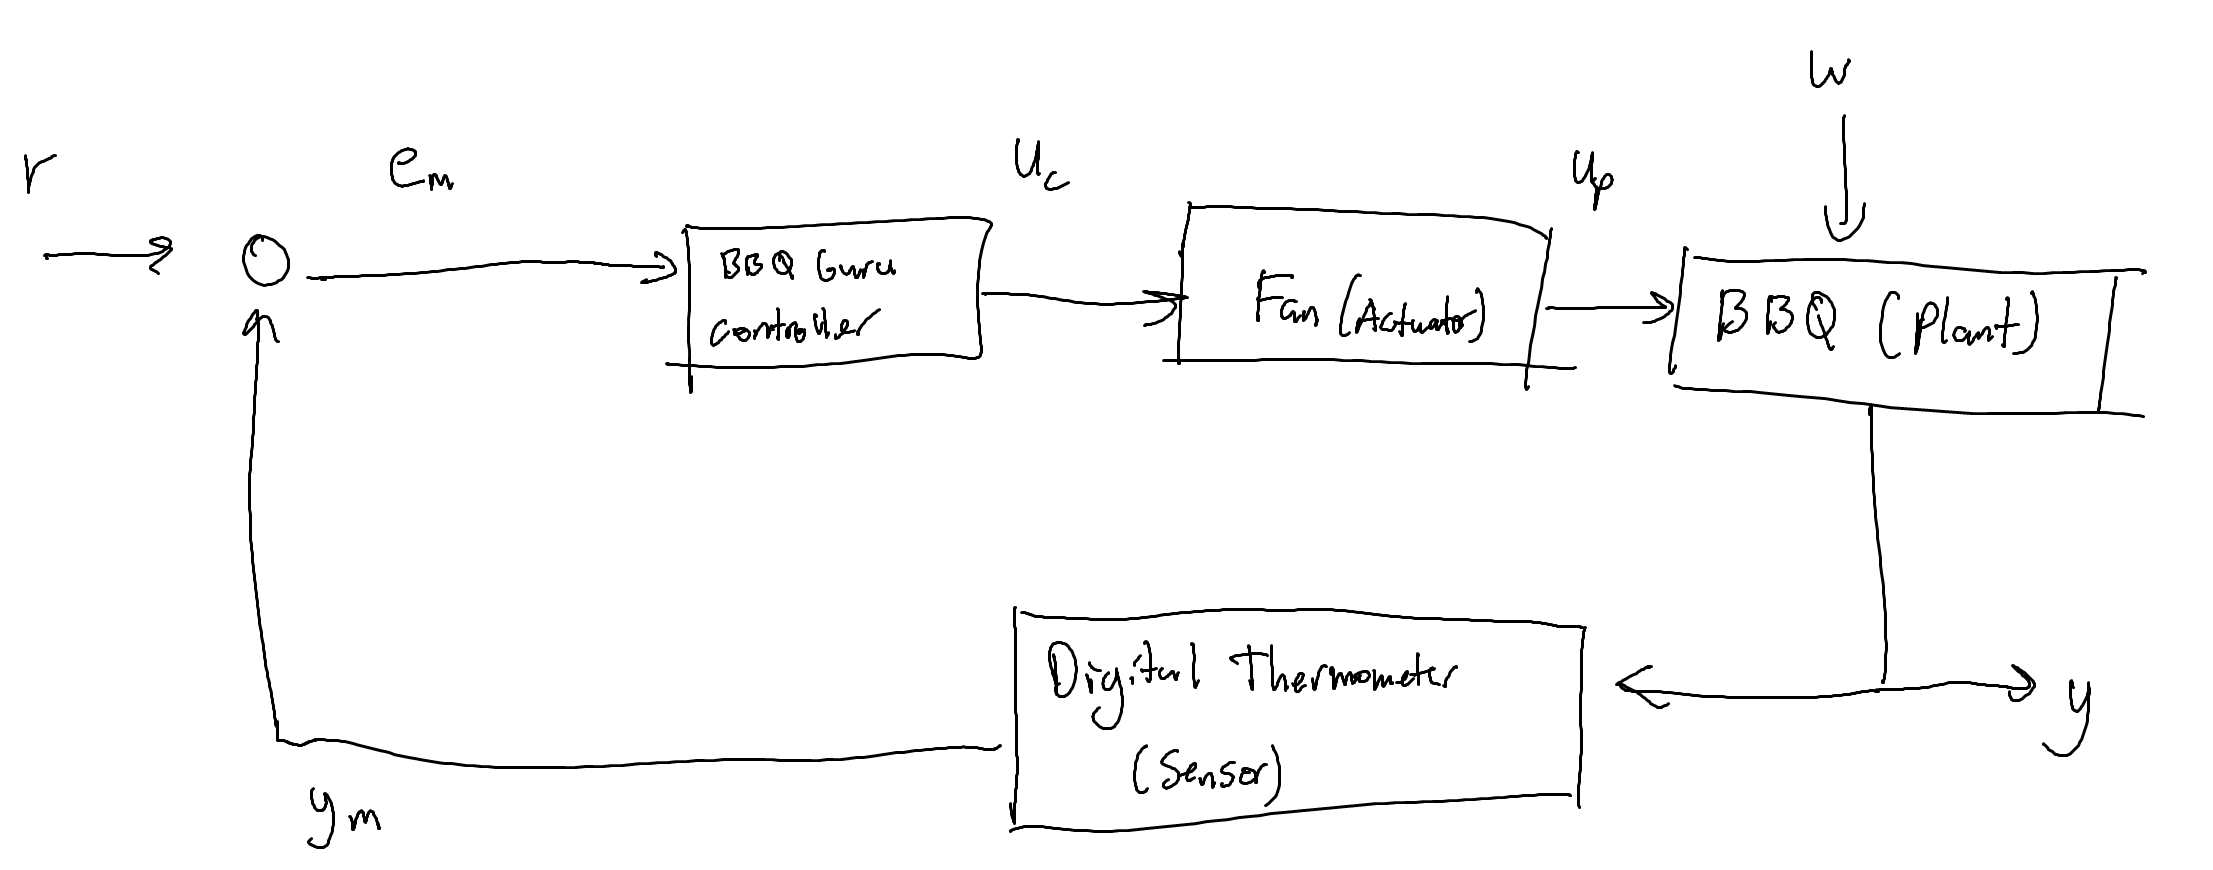
\includegraphics[width=0.8\textwidth]{Questions/Figures/Q1c.png}
    \caption{Block diagram of the overall closed-loop system for BBQ Guru.}
    \label{fig:Q1c}
\end{figure}

Where
\begin{itemize}
    \item $r$ is the reference signal, the desired temperature of the BBQ
    \item $e_m$ is the measured tracking error, the difference between the desired temperature and the measured temperature of the BBQ
    \item $u_c$ is the control input, which is the output of the controller to the fan 
    \item $u_p$ is the plant input, which is the fan speed which controls the amount of oxygen supplied to the charcoal, affecting the temperature of the BBQ
    \item $y$ is the plant output, the actual temperature of the BBQ
    \item $y_m$ is the measured plant output, the measured temperature of the BBQ from the temperature sensor as an electronic signal
    \item $w$ is the disturbance, which is the environmental factors that affect the temperature of the BBQ
    \item $v$ is the sensor noise, which is the noise from the temperature sensor
\end{itemize}

\section{}
Consider the following system consisting of two carts connected by a damper:
\begin{figure}[h]
    \centering
    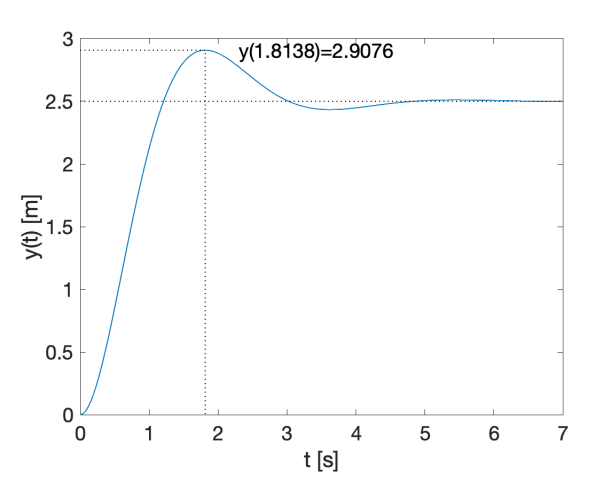
\includegraphics[width=0.5\textwidth]{Questions/Figures/Q2ProblemDiagram.png}
    \caption{System consisting of two carts connected by a damper.}
    \label{fig:Q2 System}
\end{figure}

The input is the force $F$ applied to the first cart, while $q_1$ and $q_2$ are the positions of the first and second cart, 
respectively. The output is the position of the second cart $q_2$.

\subsection{}
\textit{Using Newton’s Second Law, obtain the equations of motion of the system.}

% Figure to be included later

Since both carts are moving, the damper is applying a force based on the relative velocity of the two carts. The equation of motion for the first cart is:

\begin{equation}
    \boxed{M_1\ddot{q_1} = F - D(\dot{q_2} - \dot{q_1})} \nonumber
\end{equation}

By Newton's Third Law, the damping force on the second cart is equal and opposite to the damping force on the first cart. The equation of motion for the second cart is:

\begin{equation}
    \boxed{M_2\ddot{q_2} = D(\dot{q_2} - \dot{q_1})} \nonumber
\end{equation}

\subsection{}
\textit{Introduce the state variables $x_1 = q_1$, $x_2 = q_2$, $x_3 = \dot{q_1}$, $x_4 = \dot{q_2}$. Obtain the state model of this system.}

In addition to the above state variables, let the system input be $u = F$. The state model of this system is:

% begin empheq wiht box
\begin{empheq}[box=\fbox]{align*}
    \dot{x_1} &= x_3 \\
    \dot{x_2} &= x_4 \\
    \dot{x_3} &= \frac{1}{M_1}u - \frac{D}{M_1}(x_4 - x_3) \\
    \dot{x_4} &= \frac{D}{M_2}(x_4 - x_3) \\
    y &= x_2
\end{empheq}

\subsection{}
\textit{Obtain the state-space form of this system.}

By inspection, the state dynamics are linear, and the output is linear. Rewriting the state model in matrix form:
\begin{empheq}[box=\fbox]{align*}
    x &=
    \begin{bmatrix}
        \dot{x_1} \\
        \dot{x_2} \\
        \dot{x_3} \\
        \dot{x_4}
    \end{bmatrix}
    =
    \begin{bmatrix}
        0 & 0 & 1 & 0 \\
        0 & 0 & 0 & 1 \\
        0 & 0 & -\frac{D}{M_1} & \frac{D}{M_1} \\
        0 & 0 & \frac{D}{M_2} & -\frac{D}{M_2}
    \end{bmatrix}
    \begin{bmatrix}
        x_1 \\
        x_2 \\
        x_3 \\
        x_4
    \end{bmatrix}
    +
    \begin{bmatrix}
        0 \\
        0 \\
        \frac{1}{M_1} \\
        0
    \end{bmatrix}
    \begin{bmatrix}
        u \\
    \end{bmatrix} \\
    y &=
    \begin{bmatrix}
        0 & 1 & 0 & 0
    \end{bmatrix}
    \begin{bmatrix}
        x_1 \\
        x_2 \\
        x_3 \\
        x_4
    \end{bmatrix}
    +
    \begin{bmatrix}
        0
    \end{bmatrix}
    \begin{bmatrix}
        u \\
    \end{bmatrix}
\end{empheq}
\section{}
Consider the following closed-loop system:
% too lazy to remake the block diagram with tikz
\begin{figure}[h]
    \centering
    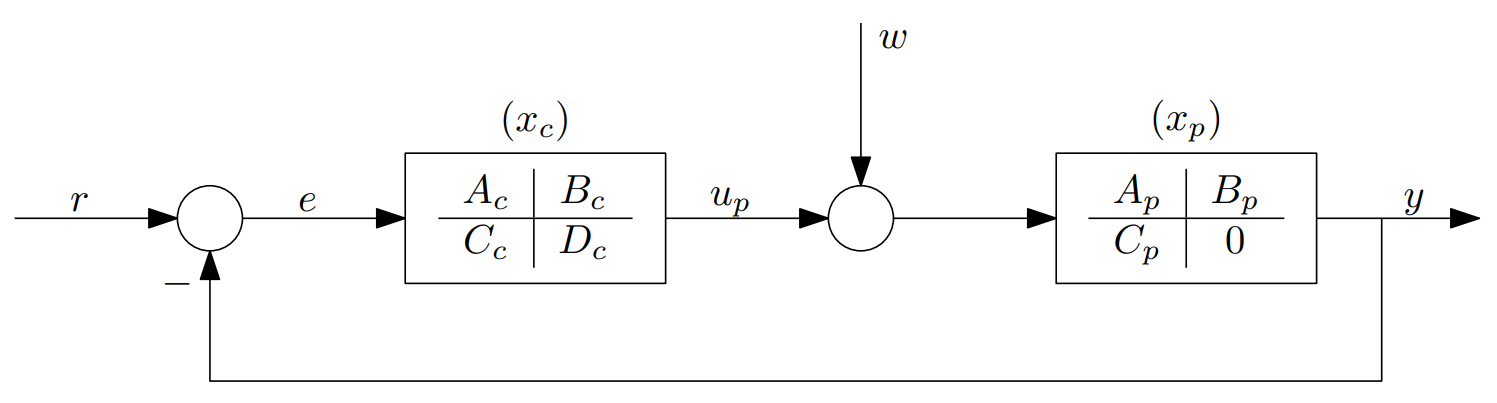
\includegraphics[width=0.5\textwidth]{Questions/Figures/Q3ProblemDiagram.png}
    \caption{Block diagram of the closed-loop system}
    \label{fig:Q3ProblemDiagram}
\end{figure}
The controller's state-space matrices are
\begin{equation*}
    A_c = -4, \quad B_c = 1, \quad C_c = -5, \quad D_c = 1
\end{equation*}
and the plant's are
\begin{equation*}
    A_p = \begin{bmatrix}
        0 & 1 \\
        -2 & -3
    \end{bmatrix}, \quad
    B_p = \begin{bmatrix}
        1 \\
        0
    \end{bmatrix}, \quad
    C_p = \begin{bmatrix}
        1 & 0
    \end{bmatrix}
\end{equation*}
\begin{enumerate}[label=(\alph*)]
    \item Form the closed-loop system dynamics matrix $A_{cl}$. Verify the internal stability of the system.
    \item Convert the state-space control and plant blocks into transfer functions $G_c(s)$ and $G_p(s)$, then form the characteristic polynomial. Verify the input-output stability of the system (note you can either compute the roots numerically, or use the Routh-Hurwitz criterion)
    \item What's the relationship between the results in (a) and (b)?
\end{enumerate}

\subsection{}
% \subsection{Closed Loop Stability}
% \begin{figure}[h]
%     \centering
%     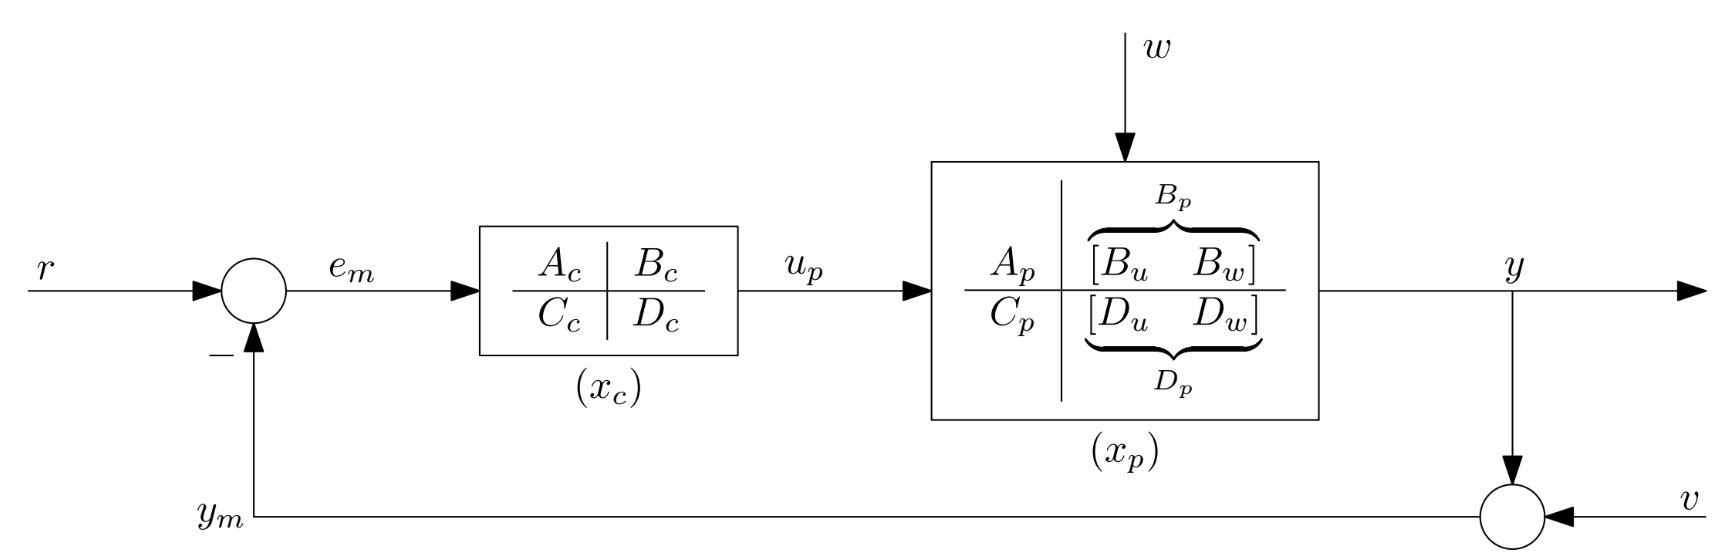
\includegraphics[width=0.5\textwidth]{closed loop diagram.png}
%     \caption{Closed loop system}
% \end{figure}
% Assume:
% \begin{itemize}
%     \item Both controller ($A_c$, $B_c$, $C_c$, $D_c$) and plant ($A_p$, $B_p$, $C_p$, $D_p$) are minimal realizations.
%     \item $D_c= 0$ or $D_p = [D_u, D_w] = 0$, such that $D_c D_u = D_u D_c = 0$ and $D_c D_w = D_w D_c = 0$.
% \end{itemize}
% Then, the state-space form of the closed loop system is:
% \begin{align*}
%     \dot{x}_cl &= \begin{bmatrix}
%         \dot{x}_c \\
%         \dot{x}_p
%     \end{bmatrix} = \underbrace{
%     \begin{bmatrix}
%     A_c - B_c D_u C_c & -B_c C_p \\
%     B_u C_c & A_p - B_u D_c C_p
%     \end{bmatrix}}_{A_{cl}}
%     \begin{bmatrix}
%         x_c \\
%         x_p
%     \end{bmatrix} + \underbrace{
%     \begin{bmatrix}
%         B_c & -B_c D_w & -B_c \\
%         B_u D_c & B_w & -B_u D_c
%     \end{bmatrix}}_{B_{cl}}
%     \begin{bmatrix}
%         r \\
%         w \\
%         v 
%     \end{bmatrix} \\
%     y_cl &= \begin{bmatrix}
%         e_m \\
%         u_p \\
%         y  \\
%         y_m 
%     \end{bmatrix} = \underbrace{
%     \begin{bmatrix}
%         -D_u C_c & -C_p \\
%         C_c & -D_c C_p \\
%         D_u C_c & C_p \\
%         D_u C_c & C_p 
%     \end{bmatrix}}_{C_{cl}}
%     \begin{bmatrix}
%         x_c \\
%         x_p
%     \end{bmatrix} + \underbrace{
%     \begin{bmatrix}
%         1 & -D_w & -1 \\
%         D_c & 0 & -D_c \\
%         0 & D_w & 0 \\
%         0 & D_w & 1
%     \end{bmatrix}}_{D_{cl}}
%     \begin{bmatrix}
%         r \\
%         w \\
%         v
%     \end{bmatrix}
% \end{align*}
To be able to use the developments in the notes, two assumptions have to be satisfied:
\begin{itemize}
    \item Both controller ($A_c$, $B_c$, $C_c$, $D_c$) and plant ($A_p$, $B_p$, $C_p$, $D_p$) are minimal realizations.
    \item $D_c= 0$ or $D_p = [D_u, D_w] = 0$, such that $D_c D_u = D_u D_c = 0$ and $D_c D_w = D_w D_c = 0$. This is satisfied in this case, since $D_p = 0$.
\end{itemize}
Then, the state-space form of the closed loop system is calculated by Matlab:
\begin{verbatim}
>> Gc
 
Gc =
 
1 - 5/(s + 4)
 
>> Gp
 
Gp =
 
(s + 3)/(s^2 + 3*s + 2)
\end{verbatim}

Both $G_c(s)$ and $G_p(s)$ are minimal realizations, so the derivations in the notes can be used.
\begin{align*}
    A_cl = \begin{bmatrix}
        A_c & -B_c C_p \\
        B_u C_c & A_p - B_u D_c C_p
    \end{bmatrix} 
\end{align*}
Employing Matlab again,
\begin{verbatim}
Acl =

    -4    -1     0
    -5    -1     1
     0    -2    -3


V =

   -0.5774    0.2145    0.1345
   -0.5774   -0.7762   -0.1859
   -0.5774    0.5929    0.9733


D =

   -5.0000         0         0
         0   -0.3820         0
         0         0   -2.6180

Real part of eigenvalues of Acl: 

ans =

   -5.0000         0         0
         0   -0.3820         0
         0         0   -2.6180
\end{verbatim}

\textbf{Since all the eigenvalues of $A_{cl}$ have negative real parts, the closed-loop system is internally stable.}

All Matlab calculations can be found in the script:
\lstinputlisting[language=Matlab]{Questions/Code/a6q3a.m}

\subsection{}

\section{}
Consider the Laplace Transform of $f(t)$ given by
\[
    F(s) = \frac{16s^2 + 23s + 13}{(s + 1)^2(s + 2)}
\]

\begin{enumerate}[label=(\alph*)]
    \item What are the poles of $F(s)$?
    \item Using the Final Value Theorem, predict the behaviour of $f(t)$ as $t \to \infty$
    \item By hand, obtain the partial fraction expansion of $F(s)$
    \item Use MATLAB's \texttt{partfrac} to confirm your result; provide the input commands you used.
    \item Obtain $f(t)$, and confirm the prediction from (b) holds. Hint: $\lim_{t \to \infty} te^{-t} = 0$
\end{enumerate}

\subsection{}
The poles of $F(s)$ are $s = -1$ and $s = -2$. The pole at $s = -1$ has a multiplicity of 2.

\subsection{}
Using the Final Value Theorem, we can see the contribution of each pole.

\begin{enumerate}
    \item $s = -1$ has a multiplicity of 2, so the contribution will be $e^{-t}$ and $te^{-t}$.
    \item $s = -2$ has a multiplicity of 1, so the contribution will be $e^{-2t}$.
\end{enumerate}

Therefore, as $t \to \infty$, $f(t) \to 0$. This is statement 3 of the Final Value Theorem in the course notes.

\subsection{}
By the Heaviside Cover-up Method, we can obtain the partial fraction expansion of $F(s)$.

\[
\begin{aligned}
    F(s) &= \frac{16s^2 + 23s + 13}{(s + 1)^2(s + 2)} \\
    &= \frac{A}{s + 1} + \frac{B}{(s + 1)^2} + \frac{C}{s + 2} \\
    &= \frac{A(s + 1)(s + 2) + B(s + 2) + C(s + 1)^2}{(s + 1)^2(s + 2)} \\
    &= \frac{(A + C)s^2 + (3A + 2B + 2C)s + (2A + B + C)}{(s + 1)^2(s + 2)}
\end{aligned}
\]

By cover-up,
\[
\begin{aligned}
    B &= \frac{16s^2 + 23s + 13}{(s + 2)} \bigg|_{s = -1} \\
    &= \frac{16(-1)^2 + 23(-1) + 13}{(-1 + 2)} \\


\]

Solving this system of equations, we get $A = 3$, $B = 2$, and $C = 13$.

\subsection{}
Using MATLAB's \texttt{partfrac} command, we get the following result.

\begin{verbatim}
>> partfrac(16*s^2 + 23*s + 13, (s + 1)^2*(s + 2))

ans =

     3/(s + 1) + 2/(s + 1)^2 + 13/(s + 2)
\end{verbatim}

\subsection{}
Using the inverse Laplace Transform, we get the following result.

\begin{align*}
    f(t) &= \mathcal{L}^{-1} \left\{ \frac{16s^2 + 23s + 13}{(s + 1)^2(s + 2)} \right\} \\
    &= \mathcal{L}^{-1} \left\{ \frac{3}{s + 1} + \frac{2}{(s + 1)^2} + \frac{13}{s + 2} \right\} \\
    &= \mathcal{L}^{-1} \left\{ \frac{3}{s + 1} \right\} + \math

% \newpage
% %\bibliographystyle{IEEEtran}
% %\bibliography{citations.bib}
% %\bibliography{}

% \newpage
% \appendix
% \sectionfont{\large}
\section{Appendix: Matplotlib Python Code to Render Graphs}
This is just some random code.
\begin{lstlisting}[language=Python]
if transactions: Transaction.create_transactions() # if transactions = "true"
node.generate_emptyState() # empty state for all nodes
S.initial_events() # initiate initial events to start with

while not queue.isEmpty() and clock <= targetTime:
    next_e = queue.get_next_event()
    clock = next_e.time # move clock to the time of the event
    Event.execute_event(next_e)
    Queue.remove_event(next_e)

print results
\end{lstlisting}

\end{document}